%! Author = Len Washington III
%! Date = 10/2/24

% Preamble
\documentclass[
	chapter=5,
	title={Gases},
	showanswers=true,
]{chem122notes}

% Packages

% Document
\begin{document}

\section{Characteristics of Gases}\label{sec:characteristics-of-gases}
\begin{itemize}
	\item Gas molecules are very far apart, so total volume of gases is mostly empty space.
	\item Gas molecules move at high velocities and high kinetic energies.
	\item Gas volume is dependent on pressure, temperature and moles of the gas.
\end{itemize}

\section{Real Gases and Ideal Gases}\label{sec:real-gases-and-ideal-gases}
\begin{itemize}
	\item Real gases obey the laws of ``ideal'' gases at non-extreme conditions.
	\item Therefore, gas behavior (pressure, temperature, volume, and number of particles) is determined using gas laws.
\end{itemize}

\section{Pressure}\label{sec:pressure}
\begin{itemize}
	\item Pressure is the force per unit area.
	\begin{equation}
		P = \frac{Force}{Area} \ \ or\ \ P = \frac{F}{A}\\
		\label{eq:pressure}
	\end{equation}
	\item So, the pressure will increase with a greater force exerted on an area or with a certain force exerted on a smaller area.
\end{itemize}

\section{Measuring Pressure}\label{sec:measuring-pressure}
\begin{minipage}[m]{0.7\textwidth}
	\begin{itemize}
		\item A barometer is one way to measure pressure.
		\item The height of the mercury column in the tube correlates to the atmospheric pressure.
	\end{itemize}
\end{minipage}\hfill%
\begin{minipage}[m]{0.3\textwidth}
	% TODO: Insert the image
\end{minipage}

\section{Pressure Units}\label{sec:pressure-units}
\begin{itemize}
	\item There are several different units used to describe pressure. We will focus on four of them:
	\begin{description}[font=\bfseries]
		\item[atm] atmospheres
		\item[mmHg] millimeters of Mercury
		\item[torr]
		\item[psi] pounds per square inch
	\end{description}
	\item 1 atm = 760 mmHg, 1 atm = 760 torr, and 1 atm = 14.7 psi
	\item So 1 mmHg = 1 torr.
	\begin{itemize}
		\item Note: atm, mmHg, and torr are all exact values; psi has been rounded to three sig figs.
	\end{itemize}
\end{itemize}

\section{Examples}\label{sec:examples}
\begin{enumerate}[label=\arabic*.]
	\item A tire pressure gauge reads 33 psi. What is this pressure reading in torr?%
	\begin{answer}
		\begin{equation*}
		\begin{aligned}
			33 \mbox{ psi} \times \frac{1 \mbox{ atm}}{14.7 \mbox{ psi}} \times \frac{\mbox{760 torr}}{ \mbox{1 atm}} = 1,\underline{7}06.12245 \mbox{ torr}
		\end{aligned}
		\end{equation*}
	\end{answer}
	\item In a near-vacuum, the pressure is 0.100 mmHg. What is this pressure in atmospheres?%
	\begin{answer}
		\begin{equation*}
		\begin{aligned}
			0.100 \mbox{ mmHg} \times \frac{1 \mbox{ atm}}{760 \mbox{ mmHg}} = 1.31579 \times 10^{-4} \mbox{ atm}
		\end{aligned}
		\end{equation*}
	\end{answer}
\end{enumerate}

\section{Temperature}\label{sec:temperature}
\begin{itemize}
	\item One factor involved in gas behavior is temperature (a measure of hot and cold).
	\item In the lab, temperature is measured in \textdegree{}C, but in gas law problems, the temperature needs to be in Kelvin (K)
	\begin{equation}
		\textdegree K = \textdegree C+ 273.15
		\label{eq:kelvin-conversion}
	\end{equation}
	\item \textbf{Lecture Problem:} A gas is collected in the laboratory at 34\textdegree{}C\@. What is the temperature on the Kelvin scale?
	\begin{answer}
		34\textdegree{}C + 273.15 = 307.15\textdegree K
	\end{answer}
\end{itemize}

\section{The Gas Laws}\label{sec:the-gas-laws}
\begin{itemize}
	\item The Gas Laws focus on the relationship between pressure, temperature, volume, and the amount of a gas.
	\item We will discuss four gas laws in these sections: \hyperref[sec:boyles-law]{Boyle's Law}, \hyperref[sec:charles-law]{Charles' Law}, \hyperref[sec:amontons-law]{Amonton's Law}, and the \hyperref[the-combined-gas-law]{Combined Gas Law}.
	\item Note: Any references to standard temperature and pressure (STP\label{dfn:stp}) means 273 \textdegree{}K and 1 atm.
\end{itemize}

\section{Boyle's Law}\label{sec:boyles-law}
\begin{itemize}
	\item If the temperature and amount of a gas are held constant, then the volume of a gas will be inversely proportional to its pressure.
\end{itemize}
\begin{equation}
	\mbox{\textbf{P}}\uparrow\mbox{\textbf{V}}\downarrow \mbox{  and  } \mbox{\textbf{P}}\downarrow\mbox{\textbf{V}}\uparrow
	\label{eq:boyles-law}
\end{equation}

\subsection{Boyle's Law Mathematically}\label{subsec:boyle's-law-mathematically}
Since volume and pressure are inversely proportional to each other, then the mathematical relationship would be:
\[ V = \frac{k}{P} \mbox{  or  } PV = k \mbox{   where } k \mbox{ is a constant.} \]
If $PV$ is a constant then we can compare how $P$ and $V$ change.
\begin{equation}
	P_{1}V_{1} = P_{2}V_{2}
	\label{eq:boyles-law-mathematically}
\end{equation}

\section{Charles' Law}\label{sec:charles-law}
If the pressure and amount of a gas is held constant, then the volume of a gas will be directly proportional to its absolute temperature (temp. in Kelvin).
\begin{equation}
	\mbox{\textbf{T}} \downarrow \mbox{\textbf{V}} \downarrow \mbox{  and  } \mbox{\textbf{T}} \uparrow \mbox{\textbf{V}} \uparrow
	\label{eq:charles-law}
\end{equation}

\subsection{Charles' Law Mathematically}\label{subsec:charles-law-mathematically}
Since temperature and volume are directly proportional to each other, then the mathematical relationship would be:
\[ V = kT \mbox{  or  } \frac{V}{T} = k \mbox{   where } k \mbox{ is a constant.} \]
If $\frac{V}{T}$ is a constant, then we can compare how $T$ and $V$ change.

\begin{equation}
	\frac{P_{1}}{V_{1}} = \frac{P_{2}}{V_{2}}
	\label{eq:charles-law-mathematically}
\end{equation}

\section{Amonton's Law}\label{sec:amontons-law}
If the volume and amount of a gas is held constant, then the pressure of a gas will be directly proportional to its absolute temperature (temp. in Kelvin).
\begin{equation}
	\mbox{\textbf{T}} \downarrow \mbox{\textbf{P}} \downarrow \mbox{  and  } \mbox{\textbf{T}} \uparrow \mbox{\textbf{P}} \uparrow
	\label{eq:amontons-law}
\end{equation}

\subsection{Amonton's Law Mathematically}\label{subsec:amontons-law-mathematically}
Since temperature and pressue are directly proportional to each other, then the mathematical relationship would be:
\[ P = kT \mbox{  or  } \frac{P}{T} = k \mbox{   where } k \mbox{ is a constant.} \]
If $\frac{P}{T}$ is a constant, then we can compare how $T$ and $P$ change.

\begin{equation}
	\frac{P_{1}}{T_{1}} = \frac{P_{2}}{T_{2}}
	\label{eq:amontons-law-mathematically}
\end{equation}

\section{The Combined Gas Law}\label{sec:the-combined-gas-law}
The Combined Gas Law relates pressure, temperature, and volume of a gas given that the amount of the gas remains constant.

\subsection{The Combined Gas Law Mathematically}\label{subsec:the-combined-gas-law-mathematically}
If we combine all the gas laws together, we get:
\begin{equation}
	\frac{P_{1}V_{1}}{T_{1}} = \frac{P_{2}V_{2}}{T_{2}}
	\label{eq:combined-gas-law}
\end{equation}

\section{Densities and Molar Masses of Gases}\label{sec:densities-and-molar-masses-of-gases}
\begin{itemize}
	\item The density of a gas is expressed in grams/liter.
	\item Since the volume of a gas is dependent on pressure and temperature, the pressure and temperature must be given for a specific density.
	\item At STP, 22.4 L of a gas contains one mole of the gas. This is known as the molar volume\label{dfn:molar-volume} (22.4 L/mol).
\end{itemize}

\section{Examples}\label{sec:examples-2}
\begin{itemize}
	\item Calculate the density, in g/L, of chlorine gas at STP\@.
	\item What is the molar mass of a gas having a density of 2.99 g/L at STP?
	\item The molar mass of a gas at STP is 132.5 g/mol. What is the density at 56\textdegree{}C and 1250 torr?
\end{itemize}

\section{The Ideal Gas Equation}\label{sec:the-ideal-gas-equation}
\begin{itemize}
	\item The Ideal Gas Law relates all four properties of a gas: pressure, temperature, volume, and amount (moles).
	\begin{equation*}
	\begin{aligned}
		PV = k \ \ &\ \  \frac{V}{T} = k \ \ &\ \  \frac{P}{T} = k \ \ &\ \  \frac{V}{n} = k
	\end{aligned}
	\end{equation*}
	\item If all of the above relationships are combined we get:
	\begin{equation}
		k = \frac{PV}{nT}
		\label{eq:ideal-gas-equation}
	\end{equation}
	\item For the Ideal Gas Law, the constant is $R$ (the universal gas constant, $0.0821\ \frac{L\times atm}{mol\times K}$).
	\item So $\frac{PV}{nT} = R$ or $PV = nRT$
\end{itemize}

\section{Examples}\label{sec:examples-3}
\begin{itemize}
	\item 50.0 g of \ce{N2O} is placed in a 10.0 L container. The temperature is 10.0\textdegree{}C. What is the pressure, in torr, of the gas?
\end{itemize}

\section{Mixture of gases and Partial Pressures}\label{sec:mixture-of-gases-and-partial-pressures}
For a multicomponent gas mixture (consisting of gases $a$, $b$, $c$, etc).
\[ \mbox{Partial Pressures: } P_{a} = \frac{n_{a}RT}{V}, P_{b} = \frac{n_{b}RT}{V}, P_{c} = \frac{n_{c}RT}{V}, \dots \]

Dalton's Law of Partial Pressures:
\begin{equation}
	\begin{aligned}
		P_{total} &= P_{a} + P_{b} + P_{c} + \dots\\
				  &= \frac{n_{a}RT}{V} + \frac{n_{b}RT}{V} + \frac{n_{c}RT}{V} + \dots\\
				  &= \frac{RT}{V}\left( n_{a} + n_{b} + n_{c} + \dots \right)\\
				  &= \frac{RT}{V}n_{total}\\
		\frac{P_{a}}{P_{total}} &= \frac{\frac{n_{a}RT}{V}}{n_{total} \times \frac{RT}{V}}\\
								&= \frac{n_{a}}{n_{total}}\\
								&= X_{a} \mbox{  (mole fraction)}\\
		P_{a} &= X_{a}P_{total}
	\end{aligned}
	\label{eq:daltons-law}
\end{equation}

\section{Gas Stoichiometry}\label{sec:gas-stoichiometry}
How many grams of water form when 1.24 L of \ce{H2} gas at STP completely reacts with \ce{O2}?
\centerce{2H2(g) + O2(g) -> 2H2O(g)}
\begin{answer}
	\begin{equation*}
	\begin{aligned}
		1.24 \mbox{ L } \ce{H2} \times \frac{1 \mbox{ mol } \ce{H2}}{22.4 \mbox{ L } \ce{H2}}
	\end{aligned}
	\end{equation*}
\end{answer}

\section{Kinetic Molecular Theory: A Model for Gases}\label{sec:kinetic-molecular-theory}
In this theory, a gas is modeled as a collection of particles (either molecules or atoms, depending on the gas) in constant motion.
A single particle moves in a straight line until it collides with another particle (or with the container wall).
Kinetic molecular theory has 3 basic postulates (assumptions)
\begin{enumerate}
	\item\label{pos:kmt-1} The size of a particle is negligibly small: the particles themselves occupy no volume, even though they have mass
	\item\label{pos:kmt-2} The average kinetic energy of a particle is proportional to the temperature in K: $KE \propto T$.
	\item\label{pos:kmt-3} The collision of one particle with another (or with the walls) is completely elastic.
	This means that when two particles collide, they may exchange energy, but there is no overall loss of energy.
	Any kinetic energy lost by one particle is completely gained by the other.
	\begin{itemize}
		\item The ideal gas law follows directly from the kinetic molecular theory, validating the latter, at least under conditions where the ideal gas law works.
		\item The concept of pressure and each fo the gas laws follows conceptually from the kinetic molecular theory.
	\end{itemize}
\end{enumerate}

\section{The Nature of Pressure}\label{sec:the-nature-of-pressure}
As each particle collides with a surface, it exerts a force upon that surface.
The result of many particles in a gas sample exerting forces on the surfaces around them is a constant pressure.

\subsection{Boyle's Law}\label{subsec:nature-of-pressure-boyles-law}
Boyle's law states that, for a constant number of particles at constant temperature, the volume of a gas is inversely proportional to its pressue.
If we decrease the volume of a gas, we force the gas particles to occupy a smaller space.
It follows from the kinetic molecular theory that, as long as the temperature remains the same, the result is a greater number of collisions with the surrounding surfaces and therefore a greater pressure.

\subsection{Charles' Law}\label{subsec:nature-of-pressure-charles-law}
Charles' Law states that, for a constant number of particles at constant pressure, the volume of a gas is proportional to its temperature (in K).
According to the kinetic molecular theory, when we increase the temperature of a gas, the average speed, and thus the average kinetic energy of the particles increases.
Since this greater kinetic energy results in more frequent collisions and more force per collision, the only way for the pressure to remain constant is for the volume to increase.
The greater volume spreads the collision out over a greater area, so that the pressure $\frac{F}{A}$ in unchanged.

\section{Avogadro's Law}\label{sec:avogadros-law} % TODO: Check if Amonton's Law should be Avogadro's Law
Avogadro's Law states that, at constant temperature and pressure, the volume of a gas is proportional to the number of particles.
According to the kinetic molecular theory, when we increase the number of particles in a gas sample, the number of collisions with the surrounding surfaces increases.
Since the greater number of collisions would result in a greater overall force on surrounding surfaces, the only way for the pressure to remain constant is for the volume to increase so that the number of particles per unit volume (and thus the number of collisions) remains constant.

\section{Temperature and Molecular Velocities}\label{sec:temperature-and-molecular-velocities}
\begin{itemize}
	\item The kinetic energy (KE) of a particle is $\frac{1}{2}mv^{2}$ where $m$ is the mass of the particle and $v$ is the velocity of the particle (KE is the integral of momentum $mv$).
	\item In a gas mixture at a given temperature, lighter particles travel faster (on average) than heavier ones.
	\item Root mean square velocity $u_{rms} = \sqrt{\vec{u}^{2}}$ where $\vec{u}^{2}$ is the average of the squares of the particle velocities.
	\item $u_{rms}$ is conceptually similar to average velocity, but not identical
	\item Average KE of one mole of gas particles:
	\begin{equation}
		KE_{avg} = \frac{1}{2}N_{A}m\vec{u}^{2} % TODO: There's no squared here in the notes but it's used later.
		\label{eq:gas-particles-KE}
	\end{equation}
	where $N_{A}$ is Avogadro's number and $m$ is the mass of each particle.
	\item From \hyperref[pos:kmt-2]{postulate 2} of the Kinetic Molecular Theory, the average kinetic energy is proportional to the temperature in K\@.
	The proportionality constant is $\frac{3}{2}R$.
	\begin{equation}
		KE_{avg} = \frac{3}{2}RT \mbox{    (for 1 mole)}
		\label{eq:average-ke}
	\end{equation}
	where $R$ is the gas constant in different units $R \Rightarrow 8.314 \frac{\mbox{J}}{\mbox{mol}\times\mbox{K}}$
	\begin{equation*}
	\begin{aligned}
		\frac{1}{2}N_{A}m\vec{u} &= \frac{3}{2}RT\\
		\vec{u}^{2} &= \frac{3RT}{N_{A}m}\\
				&= \frac{3RT}{\mu}\\
		\vec{u}^{2} &= u_{rms}\\
					&= \sqrt{\frac{3RT}{\mu}}
	\end{aligned}
	\end{equation*}
	where $\mu$ is the molar mass in kg/mol.
\end{itemize}

\begin{figure}[H]
	\centering
	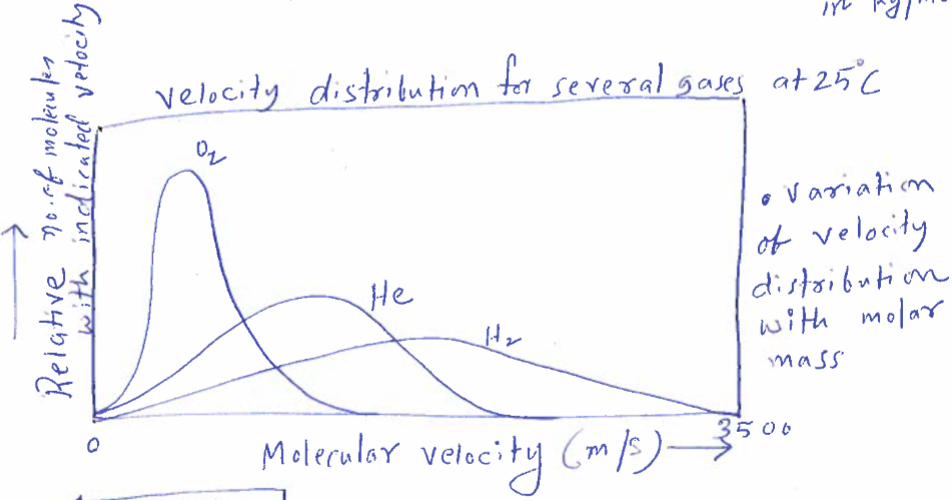
\includegraphics[width=\textwidth]{chapter6/velocity_distributions}
	\caption{Velocity distributions for several gases at 25\textdegree{}C}
	\label{fig:gas-velocity-distributions}
\end{figure}

\begin{figure}[H]
	\centering
	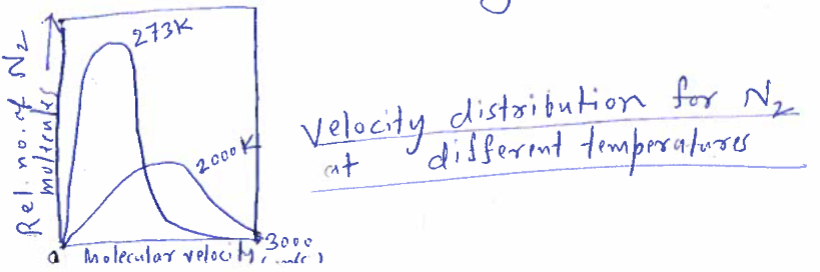
\includegraphics[width=\textwidth]{chapter6/velocity_distributions_temperatures}
	\caption{Velocity distributions for \ce{N2} at different temperatures}
	\label{fig:N2-velocity-distributions}
\end{figure}

\section{Diffusion and Effusion}\label{sec:diffusion-and-effusion}
\begin{itemize}
	\item The process by which gas molecules spread out in response to a concentration gradient is \emph{diffusion}.
	\item Heavier molecules diffuse more slowly than lighter ones, so the first molecules you smell from a perfume mixture are the lighter ones.
	\item A process related to diffusion is \emph{effusion}, the process by which a gas escapes from a container into a vacuum through a small hole.
	\item Heavier molecules effuse more slowly than lighter ones.
	\item Graham's law of effusion
	\begin{equation}
		\frac{\mbox{rate } A}{\mbox{rate } B} = \sqrt{\frac{\mu_{B}}{\mu_{A}}}
		\label{eq:grahams-law-of-effusion}
	\end{equation}
	where rate $A$ and rate $B$ are effusion rates of gases $A$ and $B$ and $\mu_{A}$ and $\mu_{B}$ are their molar masses.
\end{itemize}

An unknown gas effuses at a rate that is 0.462 times that of \ce{N2} gas (at the same temperature).
Calculate the molar mass of the unknown gas in g/mol.
\begin{answer}
	\begin{equation*}
	\begin{aligned}
		\frac{\mbox{rate unknown}}{\mbox{rate } \ce{N2}} &= \sqrt{\frac{\mu_{\ce{N2}}}{\mu_{\mbox{unknown}}}}\\
		\frac{\mbox{rate unknown}^{2}}{\mbox{rate } \ce{N2}^{2}} &= \frac{\mu_{\ce{N2}}}{\mu_{\mbox{unknown}}}\\
		\frac{\mbox{rate unknown}^{2}\times \mu_{\mbox{unknown}}}{\mbox{rate } \ce{N2}^{2}} &= \mu_{\ce{N2}}\\
		\mu_{\mbox{unknown}} &= \frac{\mu_{\ce{N2}} \times \mbox{rate } \ce{N2}^{2}}{\mbox{rate unknown}^{2}} \div \frac{\mbox{rate } \ce{N2}^{2}}{\mbox{rate } \ce{N2}^{2}}\\
							 &= \frac{\mu_{\ce{N2}}}{\left( \frac{\mbox{rate unknown}}{\mbox{rate } \ce{N2}} \right)^{2}}\\
							 &= \frac{28.08 \mbox{ g/mol}}{\left( 0.462 \right)^{2}}\\
							 &\approx 131 \mbox{ g/mol}\\
	\end{aligned}
	\end{equation*}
	The unknown gas is most likely Xenon.
\end{answer}

\section{Real Gases: The Effects of Size and Intermolecular Forces}\label{sec:real-gases}
Ideal behavior:
\begin{equation}
	V = \frac{nRT}{P}
	\label{eq:ideal-gas-behavior-volume}
\end{equation}

Corrected for volume of gas particles:
\begin{equation}
	\begin{aligned}
		V &= \frac{nRT}{P} + nb\\
		V - nb &= \frac{nRT}{P}\\
	\end{aligned}
	\label{eq:ideal-gas-behavior-with-particle-volumes}
\end{equation}
where $n$ is the number of particles and $b$ is a constant depending on the gas.

Ideal behavior:
\begin{equation}
	P = \frac{nRT}{V}
	\label{eq:ideal-gas-behavior-pressure}
\end{equation}

Corrected for intermolecular forces:
\begin{equation}
	\begin{aligned}
		P &= \frac{nRT}{V} - a\left( \frac{n}{V} \right)^{2}\\
		P + a\left( \frac{n}{V} \right)^{2} &= \frac{nRT}{V}\\
	\end{aligned}
	\label{eq:ideal-gas-behavior-with-intermolecular-forces}
\end{equation}

VanderWaals Equation show the corrected equation with the correction for intermolecular forces and particle volumes:
\begin{equation}
	\left[ P + a\left( \frac{n}{V} \right)^{2} \right] \times \left[ V - nb \right] = nRT
	\label{eq:vanderwaals}
\end{equation}

\subsection{Conditions for Ideal Behaviors of Gases}\label{subsec:conditions-for-ideal-behaviors-of-gases}
\begin{enumerate}
	\item Volume of gas particles is negligible compared to the space between them
	\item Forces between the gas particles are not significant.
\end{enumerate}


\end{document}
